\section{Modellierung}


\subsection{Hochregal}
Das gesamt Hochregallager lässt sich durch ein Objekt darstellen. Dieses Objekt enthält alle benötigten Informationen.



%
\subsection{Ereignisse}

\begin{figure}[h]
  \begin{center}
    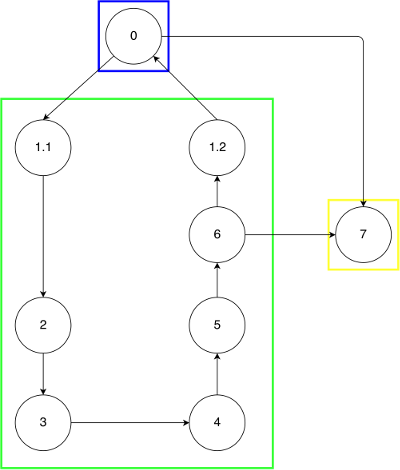
\includegraphics[width=0.5\textwidth]{images/einlagern.png}
    \caption{Einlagern}
    \label{fig:in}
  \end{center}
\end{figure}
%
\begin{figure}[h]
  \begin{center}
    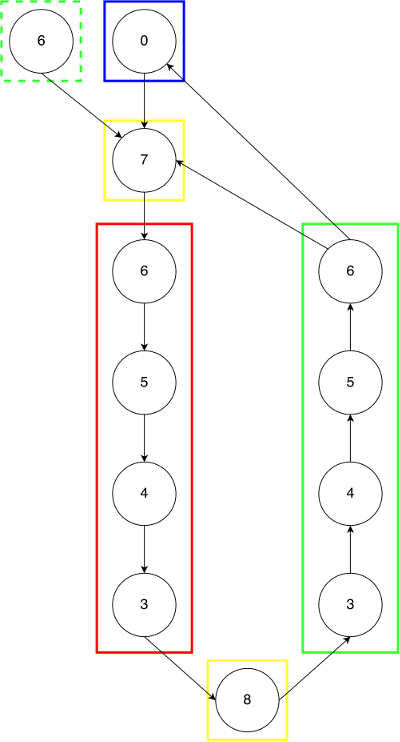
\includegraphics[width=0.5\textwidth]{images/umlagern.png}
    \caption{Umlagern}
    \label{fig:move}
  \end{center}
\end{figure}
%
\begin{figure}[h]
  \begin{center}
    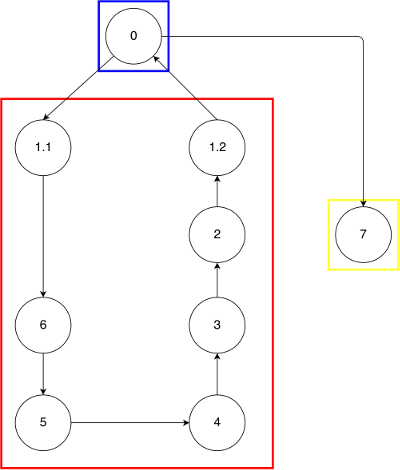
\includegraphics[width=0.5\textwidth]{images/auslagern.png}
    \caption{Auslagern}
    \label{fig:out}
  \end{center}
\end{figure}
%
\subsection{Bewegungen}





%EOF
